% Created 2023-02-07 mar 17:08
% Intended LaTeX compiler: pdflatex
\documentclass{latex/classes/thesis}
\usepackage[utf8]{inputenc}
\usepackage[T1]{fontenc}
\usepackage{graphicx}
\usepackage{longtable}
\usepackage{wrapfig}
\usepackage{rotating}
\usepackage[normalem]{ulem}
\usepackage{amsmath}
\usepackage{amssymb}
\usepackage{capt-of}
\usepackage{hyperref}
\author{Miguel Angel Piña Avelino}
\date{\today}
\title{A Study Of Concurrent Data Structures With Relaxed Semantics}
\hypersetup{
 pdfauthor={Miguel Angel Piña Avelino},
 pdftitle={A Study Of Concurrent Data Structures With Relaxed Semantics},
 pdfkeywords={},
 pdfsubject={},
 pdfcreator={Emacs 28.2 (Org mode 9.5.5)},
 pdflang={Spanish}}
\begin{document}

\maketitle
\tableofcontents


\chapter{{\bfseries\sffamily TODO} Introduction}
\label{sec:org42dc639}

\section{{\bfseries\sffamily TODO} Overview}
\label{sec:orgd05ae45}

\section{{\bfseries\sffamily TODO} Motivation}
\label{sec:orgc61d50f}

\section{{\bfseries\sffamily TODO} Objectives and contributions}
\label{sec:orge5ac9a4}

\section{{\bfseries\sffamily TODO} Organization}
\label{sec:org717efa6}

\chapter{{\bfseries\sffamily TODO} Concurrent Computing}
\label{sec:org433370b}

What is concurrent computing? This is a good question. We should first talk
about single-core and multi-core processors manufactured by the computer
industry. After the second world war and until the 90's the general purpose
cpus were single-core. All processes were executed in a single-core, and the
operating systems simulated concurrency using schedulers and other
techniques. In 2001, IBM introduce the first multi-core processor
\cite{ibmIBM100Power}, it allows that two processors work together at a very
high bandwidth (for the epoch) with large on-chip memories and with
high-speed buses. Since then, the amount of cores in each processors has been
increasing. We must consider as well the Moore's law, loosely speaking, this
law tells us that each year more and more transistors are placed into the
same space (i.e. electronic components and circuits are reduced in size), but
their speed cannot be increased without overheating. Consequently, the
industry move to ``multi-core'' architectures. In this architecture multiple
processors communicate through shared memory (RAM, hardware caches),
permitting make computing more effectively using \emph{parallelism}, where the
processors work together on a single task \cite{DBLP_books_daglib_0020056}.

\section{{\bfseries\sffamily TODO} Classic concurrent computing}
\label{sec:org64e85ee}

\begin{itemize}
\item[{$\square$}] Basic Definitions
\item[{$\square$}] FLP impossibility result
\item[{$\square$}] Asynchronous Shared Memory
\item[{$\square$}] Primitive Synchronization Operations and Consensus
\end{itemize}


\section{{\bfseries\sffamily TODO} Relaxed concurrent computing}
\label{sec:orgd4decbd}

\begin{itemize}
\item[{$\square$}] Relaxing the problem
\item[{$\square$}] Multiplicity preliminaries
\item[{$\square$}] Another relaxations?
\end{itemize}

\section{{\bfseries\sffamily TODO} Work-stealing}
\label{sec:orge695e75}

\begin{itemize}
\item[{$\square$}] How it works the work-stealing
\item[{$\square$}] Classic algorithms
\item[{$\square$}] Idempotent algorithms
\item[{$\square$}] Work-stealing with multiplicity
\end{itemize}

\section{{\bfseries\sffamily TODO} Data-Structures}
\label{sec:org87cb114}

\begin{itemize}
\item[{$\square$}] Queues with multiplicity
\end{itemize}

\chapter{{\bfseries\sffamily TODO} Preliminaries}
\label{sec:org4973e48}

\section{{\bfseries\sffamily TODO} Mathematical model}
\label{sec:orgbcde4bf}

\section{{\bfseries\sffamily TODO} Realistic model of computation}
\label{sec:orge3cb8d8}

We consider a standard concurrent shared memory system with \(n \ge 2\)
\emph{asynchronous} processes, \(p_0, \ldots, p_{n-1}\), which may crash at any time
during an execution. The processes communicate with each other by invoking
atomic instructions of base objects: either simple Read/Write instructions to
\textbf{atomic objects}, or more powerful \textbf{Read-Modify-Write} instructions, such as
\texttt{Test-And-Set}, \texttt{Swap} or \texttt{Compare-And-Set}.

For simplicity we assume a single multicore chip where the processes run. In
our system we consider a memory hierarchy, where we have the following
elements in the hierarchy:

\begin{itemize}
\item Cache memory
\item Memory bus
\item Main memory
\end{itemize}

In this model, each processor core may read and
write to a single shared memory space. Usually each processor core has a
cache to operate with data from the shared memory. Often, this data is
transferred through a memory bus, allowing connect the processors with the
memory. The figure \ref{fig:arch} shows a simplified view of this model. In
the sections: \hyperref[sec:org356909b]{Cache memory}, \hyperref[sec:orgc422088]{Memory bus} and \hyperref[sec:orgdfc917e]{Main memory}, we explain more in
detail the meaning of each bullet of the list.

\begin{figure}
\begin{minipage}{\linewidth}
  \includesvg[width=\linewidth]{figs/architecture}
\end{minipage}
\caption{Simplified view of a modern computer system cache architecture}
\label{fig:arch}
\end{figure}


\subsection{Cache memory}
\label{sec:org356909b}

The cache memory is a special very high-speed memory that is very close to
the processor and the processes can access it very fast. The caches are used
to reduce average latencies to access storage structures
\cite{DBLP_series_synthesis_2020Nagarajan}. In recent multicore chips, the
cache memory is divided in three levels, two private levels (L1 and L2) for
each processor and a third level (L3) that is shared by the cores. The
purpose of the first two levels is to provide fast access to data and
instructions for the processors.

Each processor use the first level of cache to get the data and instructions
to execute them, usually the access to this level of cache is very fast
respect to the access to other levels.  The second level is often more
capacious than first level and is used to store data and instructions that
are close to be executed. In the third level, this cache is shared by many
processors and is used as feeder for the L2 cache.

\subsection{Memory bus}
\label{sec:orgc422088}

Is a computer bus that allows transfer data from the primary memory to the
CPU and the cache memory. It is made up of two parts: the data bus and the
address bus. The data bus is in charge of transfer information between the
primary memory and the correspondent chipset.
The address bus is used to retrieve information about the location of stored
information.


\subsection{Main memory}
\label{sec:orgdfc917e}

Is the responsible of hold the data that CPU need to access frequently, such
as instructions or data currently being processed. The CPU can access to
this information faster than the access to secondary memory.

\subsection{Consistency Memory Model and Cache Coherence}
\label{sec:orgeda4069}

\begin{enumerate}
\item Consistency memory model
\label{sec:orgb5b8a7b}

Following the simplified view of the cache architecture, we want to have a
correct shared memory. And what this means? The correctness of the shared
memory can be separated into two sub-issues: \emph{consistency} and \emph{correctness}.

The consistency (definitions) provide rules about loads and stores (memory
reads and writes) and how they act upon memory. These definitions must take
into account the behaviour of those operations on memory through access of
multiple threads or even a single thread. The consistency models define
correct shared memory behavior in terms of loads and stores, without
reference to caches or coherence \cite{DBLP_series_synthesis_2020Nagarajan}.
Shared memory correctness is specified by a memory consistency model (or
memory model). This specifies the allowed behavior of multithreaded programs
executing with shared memory.

The most intuitive and strongest memory model is the \emph{Sequential Consistency}
(SC). Another memory model used by systems \emph{x86} and \emph{SPARC} is \emph{Total Store Order}
(TSO), motivated by the desire of use \emph{first-in-first-out} write buffers to
hold the results of committed stores before writing results to the caches.
Additional to the prior memory model, "relaxed" or "weak" memory models are
considered, because these models shows that most memory orderings in strong
models are unnecessary \cite{DBLP_series_synthesis_2020Nagarajan}.

\item Cache coherence
\label{sec:orgf21d97e}

Cache coherence protocols are used in response to solve a coherence problem
in cache. For example, a coherence problem can arise if multiple cores have
access to multiple copies of a datum, each one in a core, and at least one
them is a write access. The cache coherence protocols prevent the access to
stale data (incoherent data); this can be done using a set of rules
implemented by the distributed set of cores within a system. These
protocols use the common MOESI coherence states: modified (M), owned (O),
exclusive (E), shared (S) and invalid (I). The protocol acts like a state
machine, moving from one state to another based on the conditions of the
data and the cache memory \cite{DBLP_series_synthesis_2020Nagarajan}.
\end{enumerate}



\subsection{Memory fences}
\label{sec:org07f766d}

A memory fence is a barrier instruction that causes a CPU or compiler to
enforce a an ordering constraint on memory operations (loads and stores)
issued before and after the barrier instruction.

These instructions are necessary because most modern CPUs or compilers
employ performance optimizations, changing the order of the instructions on
one program, that could result in out-of-order execution. Normally these
optimizations are unnoticed in a single thread program, but can cause an
unpredictable behavior in concurrent programs.

For example, consider the following multi-thread program, with 2
threads, each one running in one core in a concurrent way:

Thread 1, core 1
\lstset{language=c++,label= ,caption= ,captionpos=b,numbers=none}
\begin{lstlisting}
while (z == 0);
print(y);
\end{lstlisting}

Thread 2, core 2
\lstset{language=c++,label= ,caption= ,captionpos=b,numbers=none}
\begin{lstlisting}
y = 30;
z = 1;
\end{lstlisting}

In this case, we might expect that the \texttt{print(y)} always print the number 30,
nevertheless, the compiler or the CPU could change the order of the
instructions for the thread 2, giving as result an execution where the value
for \texttt{y} is undefined and the instructions could be interleaved as follows:

\lstset{language=c++,label= ,caption= ,captionpos=b,numbers=none}
\begin{lstlisting}
z = 1; // Thread 2
while (z == 0); // Thread 1
print(y); // Thread 1
y = 30; // Thread 2
\end{lstlisting}

This execution is sequentially consistent, but is an out-of-order
execution producing an undefined result. With the use of memory barriers, we
can ensure that instructions don't be reordered. For example, our code could
be rewrite as follows:

Thread 1, core 1.
\lstset{language=c++,label= ,caption= ,captionpos=b,numbers=none}
\begin{lstlisting}
while (z == 0);
fence()
print(y);
\end{lstlisting}

Thread 2, core 2.
\lstset{language=c++,label= ,caption= ,captionpos=b,numbers=none}
\begin{lstlisting}
y = 30;
fence();
z = 1;
\end{lstlisting}


Languages as \texttt{Java} or \texttt{C++} provide instructions to establish synchronization
and ordering constraints between threads without an atomic operation. These
instructions have semantics well defined for

In the case of Java, we have static methods of the class VarHandle
(\texttt{java.lang.invoke.VarHandle}) that are refered as memory fence methods which
helps to provide fine-grained control of memory ordering. These statics
methods are \cite{varHandleJdk92017}:

\begin{description}
\item[{fullFence}] Ensures that loads and stores before the fence will not be
reordered with loads and stores after the fence. This method has memory
ordering effects compatible with
\texttt{atomic\_thread\_fence(memory\_order\_seq\_cst)}.
\item[{acquireFence}] Ensures that loads before the fence will not be reordered
with loads and stores after the fence. This method has memory ordering
effects compatible with \texttt{atomic\_thread\_fence(memory\_order\_acquire)}.
\item[{releaseFence}] Ensures that loads and stores before the fence will not
be reordered with stores after the fence. This method has memory ordering
effects compatible with \texttt{atomic\_thread\_fence(memory\_order\_release)}.
\item[{loadLoadFence}] Ensures that loads before the fence will not be
reordered with loads after the fence.
\item[{storeStoreFence}] Ensures that stores before the fence will not be
reordered with stores after the fence.
\end{description}

For C++, we have the function
\texttt{std::atomic\_thread\_fence}\cite{threadFenceCpp2020}, which establishes
memory synchronization ordering of non-atomic and relaxed atomic access, as
instructed by order, without an associated atomic operation. The type of
synchronization that can handle are the following:

\begin{itemize}
\item Fence-atomic synchronization
\item Atomic-fence synchronization
\item Fence-Fence Synchronization
\end{itemize}

And using a memory order\cite{memoryOrderCpp2020}, it can specifies how
memory accesses, including regular, non atomic memory accesses, are to be
ordered around an atomic operation. In total are six orders, from the
relaxed memory order to the sequential consistent memory order. They are:
\texttt{memory\_order\_relaxed}, \texttt{memory\_order\_consume}, \texttt{memory\_order\_acquire},
\texttt{memory\_order\_acq\_rel} and \texttt{memory\_order\_seq\_cst}. A note about
\texttt{atomic\_thread\_fence} functions, is that on x86 (x86\textsubscript{64}), these functions
issue no CPU instructions and only affect compile time code, with exception
for \texttt{std::atomic\_thread\_fence(std::memory\_order::seq\_cst)}, which issue the
full memory fence instruction \texttt{MFENCE}. For other archict



\section{{\bfseries\sffamily TODO} Data-Structures}
\label{sec:org75fdb32}

\subsection{Queues}
\label{sec:org414c73c}

\subsection{Stacks}
\label{sec:org89ec2ca}


\section{{\bfseries\sffamily TODO} Some Hardware Foundations}
\label{sec:org3f925ee}

\subsection{Cache memory}
\label{sec:orgfd8d3e6}

The cache memory

\begin{enumerate}
\item Multiple caches
\label{sec:org679bdd9}


\item Cache coherence protocols
\label{sec:orgdb98898}



\begin{enumerate}
\item MESI
\label{sec:orgf5764b1}


\item MOESI
\label{sec:orgd8973b7}
\end{enumerate}


\item Store Buffers
\label{sec:org17335d3}
\end{enumerate}


\subsection{Reordering (CPU or Compiler)}
\label{sec:org7bbeaa5}

\subsection{Memory Barriers}
\label{sec:orge0e257a}

\begin{enumerate}
\item X86 and TSO architectures
\label{sec:orge956e40}

\item Memory Fences
\label{sec:orgc5c7637}
\end{enumerate}

\subsection{Read-Modify-Write Operations}
\label{sec:orgd3049a6}

\subsection{Bibliography}
\label{sec:org6637d0b}

\begin{itemize}
\item \url{https://blog.the-pans.com/std-atomic-from-bottom-up/}
\end{itemize}

\section{{\bfseries\sffamily TODO} C++ Memory model}
\label{sec:org6aaa68d}

\subsection{Memory model basics}
\label{sec:org9e88abd}

\begin{enumerate}
\item Objects and memory locations
\label{sec:orgc962e2e}


\item Objects, memory locations, and concurrency
\label{sec:org8ec2aa1}


\item Modification orders
\label{sec:org5694c9a}
\end{enumerate}


\subsection{Atomic operations and types in C++}
\label{sec:orgaf839c9}


\begin{enumerate}
\item The standard atomic types
\label{sec:orgd650de3}

\item Operations on std::atomic\textsubscript{flag}
\label{sec:orgd7bb424}

\item Operations on std::atomic<boolean>
\label{sec:org9044568}

\item Operations on std::atomic<T*>: pointer arithmetic
\label{sec:orgea6b6b8}

\item Operations on standard atomic integral types
\label{sec:org1af3c0a}

\item The std::atomic<> primary class template
\label{sec:org20973d2}

\item Free functions for atomic operations
\label{sec:org871838f}
\end{enumerate}

\subsection{Synchronizing operations and enforcing ordering}
\label{sec:org5135e33}

\begin{enumerate}
\item The synchronization relationship
\label{sec:org0ea9afd}

\item The happens-before relationship
\label{sec:org414a712}

\item Memory ordering for atomic operations
\label{sec:org324216a}

\item Release sequences and synchronizes-with
\label{sec:org03036d4}

\item Fences
\label{sec:orge14e0b1}

\item Ordering non-atomic operations with atomics
\label{sec:orgb97603a}

\item Ordering non-atomic operations
\label{sec:orgd934a44}
\end{enumerate}


\section{{\bfseries\sffamily TODO} Guidelines for designing data-structures for concurrency}
\label{sec:org3d2597b}

\begin{itemize}
\item Ensure that no thread can see a state where the invariants of the
data-structure have been broken by the action of the another thread.

\item Take care to avoid race conditions inherent in the interface to the
data-structure by providing functions for complete operations rather than
for operations steps.

\item Pay attention to how the data-structure behaves in the presence of
exceptions to ensure that the invariants are not broken.

\item Minimize the opportunities for deadlock when using the data-structure by
restricting the scope of locks and avoiding nested locks where possible.
\end{itemize}





\chapter{{\bfseries\sffamily TODO} Work Stealing}
\label{sec:org99d3e31}

We analyze the algorithms for work-stealing described in the article Fully
Read/Write Fence Free Work-Stealing With Multiplicity, also the algorithm
called "Idempotent FIFO Work-Stealing", this because the algorithm have a
similar semantic than the prior algorithms.

\begin{figure}
\begin{minipage}{\linewidth}
  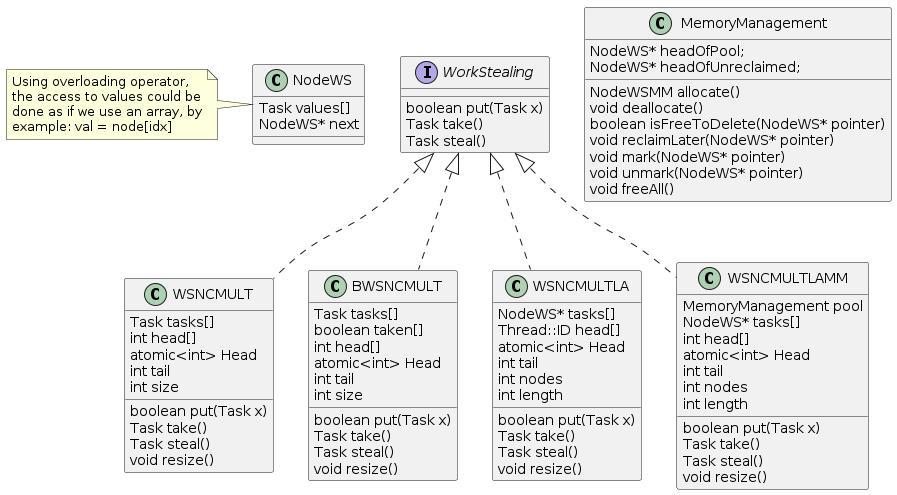
\includegraphics[width=\linewidth]{figs/objects.png}
\end{minipage}
\caption{Class Diagrama}
\label{fig:class_diagram}
\end{figure}


\section{{\bfseries\sffamily TODO} Model}
\label{sec:org47af23e}

\section{{\bfseries\sffamily TODO} Known algorithms}
\label{sec:orgd81f6af}

\section{{\bfseries\sffamily TODO} Pseudocode for Work-Stealing with Weak Multiplicity}
\label{sec:org26ea387}

\section{{\bfseries\sffamily TODO} Memory management}
\label{sec:org230d30d}

To implement efficiently the idempotent algorithms in an enviroment without
garbage collection, it's necessary use some technique or metodology to
provide garbage collection when atomic pointers are used or when distinct
threads want to reclaim the memory of the object associated to the pointer.

\begin{enumerate}
\item Strategies to delete shared pointers
\label{sec:orgc644d3d}

\begin{itemize}
\item Add pointers to list to safety delete.
\item Do this when there aren't more threads accessing to methods.
\begin{itemize}
\item Increase the counter when a thread enter to the method and decrease when
it exits.
\item Delete all pointers when the counter be equal to zero.
\end{itemize}
\end{itemize}


\item Hazard pointers
\label{sec:org86c1a75}

The \emph{Hazard Pointers} is a technique to manage memory in languages where there
are not a garbage collector. This technique was proposed by Maged
Michael \cite{DBLP_journals_tpds_Michael04}. They are so called because
deleting a pointer that might be referenced by other thread(s) is
dangerous. If another threads keep holding references to that pointer and
proceed to access to that pointer after be deleted, you have a undefined
behavior \cite{DBLP_journals_tpds_Michael04}.

The basic idea of this technique is the following:

\begin{itemize}
\item If a thread want to use a pointer that another thread might want to
delete, it first sets a hazard pointer to the pointer, informing to the
other thread that deleting the pointer would be dangerous. Once the object
is not longer needed, the hazard pointer is cleared.
\item When a thread wants to delete the pointer, it must check if the hazard
pointers belonging to the other threads in the system. If no one has a
reference to the pointer, then, it's safe to delete the
pointer. Otherwise, it must be left until later.
\item Periodically, we must check the list of objects that have been left until
later to see if any of them can be deleted now.
\end{itemize}

A general pseudocode for this technique could be the following:

\lstset{language=c++,label= ,caption= ,captionpos=b,numbers=none}
\begin{lstlisting}
void func() {
    std::atomic<void*>& hp = get_hazard_pointer_for_current_thread();
    void* old_data = data.load();
    do {
        void* temp;
        do{ // Loop until you've set the hazard pointer
            temp = old_data;
            hp.store(old_data);
            old_data = data.load();
        } while (old_data != temp);
          }while (old_data &&
            !data.compare_exchange_strong(old_data, old_data->next);
    // Do something with old_data
    hp.store(nullptr); // clearing usage of hazard pointer
    // Trying clearing
    if (outstanding_hazard_pointers_for(old_head))
    {
        reclaim_later(old_data);
    }
    else
    {
        delete old_data;
    }
    delete_nodes_with_no_hazards();
}
\end{lstlisting}


\item Atomic Smart Pointers (Herlihy, Chapter 19) (Not available for GCC and CLang)
\label{sec:org9d6caaa}


When a memory region is reclaimed, the programmer cannot know how that
region of memory will be reused or if even whether it is reused. We need a
way of developing a (general) solution to prevent the sorts of races
when a memory region is reclaimed by many threads asynchronously. We can to
do this by delaying reclamation.
Thinking in terms of pending operations on a concurrent data structure, a
sufficient condition is that \emph{memmory is only reclaimed when it is impossible
for any pending operation to access in the future}.

This property could be also achieved by \emph{reference counting}. In a reference
counted implementation of a data-structure (like a list), a counter of type
atomic<int> is associated with each node. Whenever a reference to node N is
created
\end{enumerate}


\section{{\bfseries\sffamily TODO} Memory management for work-stealing algorithms}
\label{sec:org396f1b2}

It is well known that C++ does not have a garbage collector like Java. Since
the publish of the \href{https://en.cppreference.com/w/cpp/11}{Standard C++11}, new features for memory management were
added. For example, a concurrency support library and smart pointers. These
last are used to help ensure that programs are free of memory and resources
leaks and are exception safe.

For algorithms like Chaselev\cite{circular.work.stealing},
cilk\cite{implementation_cilk5}, Idempotent FIFO and Idempotent
LIFO\cite{maged.vechev.2009}, whose specification describe the use of simple
structures and variables, we can manage them using smart pointers to avoid
problems with memory management, but in the case of Idempotent
DEQUE\cite{maged.vechev.2009}, it need to use a more complex structure to
avoid problems like the \href{https://www.stroustrup.com/isorc2010.pdf}{ABA problem}.



\chapter{{\bfseries\sffamily TODO} Modular Basket Queues}
\label{sec:org96bad19}

A modular version of the basket queues of Hoffman, Shalev and Shavit is
presented. It manipulates the head and tail using a novel object called
load-link/incremental-conditional, which can be implemented using only
READ/WRITE instructions, and admits implementations that spread
contention. This suggest that there might be an alternative to the seemingly
inherent bottleneck in previous queue implementations that manipulate the
head and the tail using \emph{read-modify-write} instructions over a single shared
register.

\section{{\bfseries\sffamily TODO} Review LL/IC implementations}
\label{sec:orga2dc273}

The specification of \texttt{LL/IC} satisfies the next properties, where the state of
the object is an integer R, initialized to zero, and assuming that any
process invokes IC only if it has invoked LL before:

\begin{description}
\item[{LL()}] Returns the current value in \(R\).
\item[{IC()}] If \(R\) has not been incremented since the last LL of the
invoking process, then do \(R = R + 1\); in any case return \texttt{OK}.
\end{description}

\section{LL/IC Implementations}
\label{sec:orgf8267eb}

\begin{description}
\item[{CAS based implementation}] It uses a shared register \(R\) initialized to
zero. \texttt{LL} first reads \(R\) and stores the value in a persistent variable
\(r_p\) of \(p\), and then returns \(r_p\). \texttt{IC} first reads \(R\) and if
that value is equals to \(r_p\), then it performs \(CAS(R, r_p, r_p +
     1)\); in any case returns \texttt{OK}.
\item[{READ/WRITE based implementation}] It uses a shared array \(M\) with \(n\)
entries initialized to zero. \texttt{LL} first reads all entries of M (in some
order) and stores the maximum value in a persistent variable \(max_p\) of
\(p\), and then returns \(max_p\). \texttt{IC} first reads all entries of \(M\),
and if the maximum among these values is equals to \(max_p\), it performs
\(\W(M[p], max_p + 1)\); in any case returns \texttt{OK}.
\item[{Mixed implementation}] It uses a shared array \(M\) with \(K < n\)
entries initialized to zero. \texttt{LL} reads all entries of \(M\) and stores the
maximum value and its index in persistent variables \(max_p\) and
\(indmax_p\). \texttt{IC} non-deterministically picks and index \(pos \in \{0, 1,
     \ldots, K - 1\} \setminus \{indmax_p\}\). If \(M[pos]\) contains a value
\(x\) less than \(max_p + 1\), then it performs \(CAS(M[pos], x, max_p +
     1)\); if the \texttt{CAS} is successful, it returns \texttt{OK}. Otherwise, it reads the
value in \(M[indmax_p]\), and if it is equals to \(max_p\), then it
performs \(CAS(M[indmax_p], max_p, max_p + 1)\); in any case, it returns
\texttt{OK}.
\end{description}

\section{{\bfseries\sffamily TODO} Basket implementations}
\label{sec:org0da3780}

\begin{description}
\item[{K-Basket from FAI and SWAP}] In this first implementation, the processes
use FAI to guarantee that at most two ``opposite'' operations ``compete''
for the same location in the shared array, which can be resolved with a
SWAP; the idea is similar to the approach in the LCRQ algorithm
\cite{ppopp2013x86queues}.
\item[{n-Basket from CAS}] Each process has a dedicated location in the shared
array where it tries to put its item when it invokes \texttt{PUT}. When a process
invokes \texttt{TAKE}, it first tries to take an item from its dedicated location,
and if it does not succeed, it randomly picks non-previously-picked
location and does the same, and repeats until takes an item or all
locations have been canceled. Since several operations might ``compete''
for the same location, CAS is needed. This implementation is reminiscent
to \emph{locally linearizable} generic data structure implementations of
\cite{DBLP_conf_concur_HaasHHKLPSSV16}.
\end{description}

\section{{\bfseries\sffamily TODO} Update experiments}
\label{sec:org02345df}

To update the experiments is necessary understand what are metrics that
allows us compare the algorithms designed for LL/IC objects and Baskets. A
common way to evaluate experimental results is the use of measurements to
understand what is the performance or the throughput of the experiments;
but, what are the meaning of performance and throughput. According to the
Cambridge Dictionary, \emph{Throughput} is the amount of work done in a particular
period of time, in other side, performance is how well someone o something
functions, works, etc. By other side, \emph{Performance} is referred to the amount
of useful work accomplished by a system. Performance usually is measured in
terms of accuracy, efficiency and speed of executing instructions. From
\cite{lilja2005measuring}, some strategies for measurement are:

\begin{description}
\item[{Event driven}] It records the information necessary to calculate the
performance metric whenever an event occurs.
\item[{Tracing}] Similarly to the previous, but, instead of recording the event
has occurred, a portion of the system is recorded to identify the event.
\item[{Sampling}] This strategy records a portion of the system in a fixed time
interval.
\item[{Indirect measurement}] This type occurs when the metric data is not
directly accessible and you must find another metric that can be measured
directly.
\end{description}

We can combine those strategies with the use of interval timers to measure
how much time take execute the program or some section of code, due this can
also provide a time basis for sampling.

In \href{https://en.wikipedia.org/wiki/Computer\_performance}{terms of computing}, the performance is refered to the amount of useful
work accomplished by a computer system. Computer performance is measured in
terms of accuracy, efficiency and speed of executing computer program
instructions. One or more of the following factor might be involved:

\begin{enumerate}
\item Short response time for a given piece of work.
\item High throughput.
\item Low utilization of computing resources.
\item High availability of a computing system.
\item High bandwidth.
\item Short data transmission time.
\end{enumerate}

To begin with a performance-analysis problem, there are three techniques
that can be used to find the desired solution:

\begin{enumerate}
\item Measurements of existing systems.
\item Simulation.
\item Analytical modeling.2
\end{enumerate}

Some benchmarks used to test concurrent queues are:

\begin{itemize}
\item enqueue - dequeue pairs:
\item 50\% enqueues
\end{itemize}

In both benchmarks, some work is added to avoid long run scenarios. This
anomaly is described in \cite{DBLP_conf_podc_MichaelS96} and to avoid it, the
work added consists in spinning a small amount of time (6 \(\mu\)s) in an
empty loop. The idea behind of this is prevent long runs of queue operations
by the same process without this being interrupted, so, this would display
an overly-optimistic performance due to the lower cache miss rate.

\section{{\bfseries\sffamily TODO} Experimental setup}
\label{sec:org2e99fa1}

To evaluate our modular queue with all its variants, we need to determine a
methodology to know their performance and the throughput of each
variant. Also, we need to compare them with other queue algorithms in the
literature to check if it is competitive. We will divide the experiments into
two categories, the first one is related to measuring the performance of the
distinct variants described previously. The second is to compare our best
queue algorithm (or the two best) to related queue algorithms in the
literature. To know the performance of our algorithms, we want to measure the
time required to execute a set of operations over an interval of time, i.e.,
how quickly complete its execution the program. The technique used to measure
the time of an event is the following:

\begin{itemize}
\item Read the current time and store it in a variable \texttt{start\_count}.
\item Let the portion of program execute.
\item Read the current time and store it in a variable \texttt{stop\_count}.
\item Take the difference between \texttt{start\_count} and \texttt{stop\_count}. This will be the
total time required to execute the event.
\end{itemize}

This technique for measuring the execution time of any portion of a program
is known as the \emph{wall clock} time\cite{lilja2005measuring}. All the events we
want to measure will use this technique to get their execution time.
However, this measurement includes the time spent on other system operations,
like memory paging, thread interleaving, input/output operations and network
communication, if applicable. Those external events could introduce
uncertainty into our measurements. We refer to these uncertainties in
measurements as errors or noise. To know how much uncertainty exists, we must
use probability and statistics tools to quantify it. To summarize a
collection of measures, we can use indices of central tendency (the mean, the
median, and the mode). The most commonly used index is the (sample
arithmetic) mean or average, which can summarize all the measurements
performed into a single number that somehow represents the center of the
distribution of these values. To quantify the precision of our measurements,
we can use a \emph{confidence interval} for the mean
value\cite{lilja2005measuring,DBLP_conf_oopsla_GeorgesBE07}. Another tools we
need are the \emph{sample variance}, the \emph{standard deviation} and the \emph{coefficient of
variation}. Formally, the \emph{(sample arithmetic) mean} is defined to be:

\begin{equation}
\bar{x}_A = \frac{1}{n}\sum^n_{i = 1}x_i
\end{equation}

Where \(x_i\) values the individual measurements. The \emph{sample variance}
represent our calculated estimated of the actual variance. It is defined to
be:

\begin{equation}
s^2 = \frac{\sum_{i = 1}^n(x_i - \bar{x}^2)}{n - 1}
\end{equation}

Where the \(x_i\) are the \(n\) independent measurements and \(\bar{x}\) is
the corresponding sample mean. From the previous equation, the standard
deviation is defined as the positive square root of the variance:

\begin{equation}
s = \sqrt{s^2} = \sqrt{\frac{\sum_{i = 1}^n(x_i - \bar{x}^2)}{n - 1}}
\end{equation}

The coefficient of variation (COV) is defined to be:

\begin{equation}
  COV = \frac{s}{\bar{x}}
\end{equation}

If we can approximate the distribution of random errors by a Gaussian
distribution, we determine how well is our estimate of the true value respect
to the actual true value using the properties of the distribution. We use
confidence intervals to find a range of values that has a given probability
of including the actual true value. For do that, we must consider two cases:

\begin{enumerate}
\item When the number of measurements is large \((n \ge 30)\).
\item When the number of measurements is small \((n < 30)\).
\end{enumerate}

For the first case, we use the sample mean \((\bar{x})\) as the best
approximation of the true value. If the \(n\) samples used to calculate
\(\bar{x}\) are all independents with mean \(\mu\) y standard deviation
\(\sigma\), the central limit theorem then assures us that, for large values
of \(n\), the sample mean \(\bar{x}\) is approximately Gaussian distributed
with mean \(\mu\) and standard deviation \(\sigma / \sqrt{n}\). We can
quantify the precision of the measurements searching two values \(c_1\) and
\(c_2\), such that the probability of the mean value being between that two
values is \(1 - \alpha\). That is \(PR[c_1 \le \bar{x} \le c_2] = 1 -
   \alpha\). \(c_1\) and \(c_2\) are chosen to form a symmetric interval around
\(\bar{x}\) such that \(Pr[x < c_1] = Pr[x > c_2] = \frac{\alpha}{2}\). The
interval \([c_1, c_2]\) is called \emph{confidence interval} for \(\bar{x}\) and
\(\alpha\) is called the \emph{significance level} and the value \((1 - \alpha)\) is
called the \emph{confidence level}. From the central-limit theorem, we have:

\begin{equation}
c_1 = \bar{x} - z_{1 - \alpha/2}\frac{s}{\sqrt{n}}
\end{equation}
\begin{equation}
c_2 = \bar{x} + z_{1 - \alpha/2}\frac{s}{\sqrt{n}}
\end{equation}


\section{{\bfseries\sffamily TODO} Experiments}
\label{sec:orgc267531}


\chapter{{\bfseries\sffamily TODO} Conclusions}
\label{sec:orgb2c1c5a}


\chapter{Material for courses}
\label{sec:org39e22c9}

\section{Introduction to multi-threading programming with Java (notes)}
\label{sec:org843edb4}
\textbf{Prerequisites to take the course}:
\begin{itemize}
\item Basic knowledge about Maven
\item An editor like emacs or vi or use an IDE like Netbeans
\item JDK 17 (open-jdk)
\item git
\end{itemize}

\subsection{Introduction}
\label{sec:org681edd2}

In the early 2000s, the multicore revolution began due to was difficulty
built processor chips smaller and faster. Derived from this situation, we had
to change the form we developing software. The multicore chips cause that
performs computing to be more effective by exploiting
``parallelism''. However, the challenge is in how to exploit that
parallelism. Those multicore chips (multiprocessors) usually use shared
memory to communicate the processors between themselves. An important aspect
when programming these multiprocessors is establishing coordination
mechanisms to access shared memory, for example, how to synchronize the
access to shared data to avoid problems while it is manipulated (writes and
lectures). The above is challenging because modern systems are inherently
asynchronous, and without synchronization mechanisms, unpredictable events
can occur while shared data is modified concurrently.

In this tutorial, we will focus on tools and techniques for programming
multiprocessors using shared memory with \texttt{Java}. We will cover some topics
related to concurrent and parallel computing.


\subsection{Processes and threads}
\label{sec:orgc1adbcf}

What is the difference between a process and a thread? Both process and
thread are independent sequences of execution. Loosely speaking, in practical
terms, a process is an executing program. A thread is a lightweight process
that can run over parallel with other threads and share resources as memory
and disc with its parent process. Usually, threads run in the process space
context.

For example, we can run a program in java (like Netbeans), and the
program in is known as the main process. During execution of program, it
can perform multiple events like calls to internet services or call to other
programs. Commonly, these events are performed in threads to avoid freeze the
main thread and are called asynchronously.

\subsection{Basics}
\label{sec:org8d63095}


\textbf{Creating the base project}: Let's create a maven based project. In a terminal,
write:

\lstset{language=bash,label= ,caption={Generating project with maven},captionpos=b,firstnumber=1,numbers=left}
\begin{lstlisting}
cd ..
mvn archetype:generate -DgroupId=mx.unam.concurrent \
    -DartifactId=concurrent-example \
    -DarchetypeArtifactId=maven-archetype-quickstart \
    -DarchetypeVersion=1.4 -DinteractiveMode=false
ls | grep concurrent-example
\end{lstlisting}

It creates a project with a main file called \texttt{App.java}. We will use that file
to write all our code for multi-threaded applications. The first thing to do
is change some parameters of our project to work with a recent java version.

In the file \texttt{pom.xml}, change the target output and compiler version. Those
values should be changed in the properties section as shown in code
\ref{orgbd8ce7f}.

\lstset{language=XML,label=orgbd8ce7f,caption={Changing content of file pom.xml},captionpos=b,firstnumber=1,numbers=left}
\begin{lstlisting}
<maven.compiler.source>17</maven.compiler.source>
<maven.compiler.target>17</maven.compiler.target>
\end{lstlisting}

However, our application still not have defined a main class used to execute
the program. To allow this, add the code shown in code \ref{orgef3ec06} to the \texttt{pom.xml},
in the plugins section.

\lstset{language=XML,label=orgef3ec06,caption={Adding a plugin to execute directly from maven},captionpos=b,firstnumber=1,numbers=left}
\begin{lstlisting}
<plugin>
  <groupId>org.codehaus.mojo</groupId>
  <artifactId>exec-maven-plugin</artifactId>
  <version>1.2.1</version>
  <executions>
    <execution>
      <goals>
        <goal>java</goal>
      </goals>
    </execution>
  </executions>
  <configuration>
    <mainClass>mx.unam.concurrent.App</mainClass>
  </configuration>
</plugin>
\end{lstlisting}

We can run our project with the following instruction:

\lstset{language=bash,label= ,caption={Example of how to execute the project},captionpos=b,firstnumber=1,numbers=left}
\begin{lstlisting}
pwd
cd ../concurrent-example
mvn compile exec:java
\end{lstlisting}


\subsection{Creating and starting a Thread}
\label{sec:orgb6e78bc}

In Java, to use threads in our applications, we can create an instance of the
class \texttt{Thread} (\texttt{java.lang.Thread}) or make a derived subclass. Also we can
provide an object that implements the \texttt{Runnable} interface
(\texttt{java.lang.Runnable}). This interface defines a single method, \texttt{run}, meant to
contain the code executed in the thread. Lets create a basic application
where we define an instance of Thread and run it.

\lstset{language=java,label= ,caption={Basic example of how to create threads},captionpos=b,firstnumber=1,numbers=left}
\begin{lstlisting}
public class App {

    public static void main(String[] args) {
        MyThread1 obj1 = new MyThread1();
        MyThread2 obj2 = new MyThread2();
        Thread t = new Thread(new MyRunnable());

        obj1.start();
        obj2.start();
        t.start();
    }
}

class MyThread1 extends Thread {
    @Override
    public void run() {
        System.out.println("Thread 1 is running");
    }
}

class MyThread2 extends Thread {
    @Override
    public void run() {
        System.out.println("Thread 2 is running");
    }
}

class MyRunnable implements Runnable {
    @Override
    public void run() {
        System.out.println("My runnable object is running");
    }
}
\end{lstlisting}

A more interesting example could be the following:

\lstset{language=java,label= ,caption={Second example of how to create threads},captionpos=b,firstnumber=1,numbers=left}
\begin{lstlisting}
package mx.unam.concurrent;

public class App {

    public static void main(String[] args) {
        MyThread1 obj1 = new MyThread1();
        MyThread2 obj2 = new MyThread2();
        Thread t = new Thread(new MyRunnable());
        obj1.start();
        obj2.start();
        t.start();
    }
}

class MyThread1 extends Thread {
    @Override
    public void run() {
        for (int i = 0; i < 10; i++) {
            String output = String.format("Thread 1 is running. Iter: %d", i);
            System.out.println(output);
        }
    }
}

class MyThread2 extends Thread {
    @Override
    public void run() {
        for (int i = 0; i < 10; i++) {
            String output = String.format("Thread 2 is running. Iter: %d", i);
            System.out.println(output);
        }
    }
}

class MyRunnable implements Runnable {
    @Override
    public void run() {
        for (int i = 0; i < 10; i++) {
            String output = String
                .format("My runnable object is running. Iter: %d", i);
            System.out.println(output);
        }
    }
}
\end{lstlisting}

A possible output for the previous code is the following. We can observe how
the calls to the \texttt{println} method are interspersed. In a sequential execution,
the output of the object \texttt{obj1} should be printed (the sequence of \texttt{printlns}
from zero to nine) followed by the output of the \texttt{obj2} (the sequence of
printlns from zero to nine) and similarly, in the end, the output from the
object \texttt{t}, but, in this, there is not a order in how the objects are
called.

\subsection{Thread managment}
\label{sec:org28d9727}

After seeing how to use threads in a basic way, now let us discuss some
methods available to thread management. More documentation about these
methods is available on
\url{https://docs.oracle.com/en/java/javase/17/docs/api/java.base/java/lang/Thread.html}.
The methods that we refer are:

\begin{itemize}
\item start
\item suspend
\item stop
\item sleep
\item join
\end{itemize}

We will exemplify the use of the first four methods using the program shown
in the code \ref{orgf8f645f}.

\lstset{language=java,label=orgf8f645f,caption={Code example using methods for control threads.},captionpos=b,firstnumber=1,numbers=left}
\begin{lstlisting}
public class App {
    public static void main(String[] args) {
        MyThread t1 = new MyThread("First Thread");
        MyThread t2 = new MyThread("Second Thread");
        try {
            Thread.sleep(500); // Sleeping for 500ms
            t1.stop();
            t2.stop();
            Thread.sleep(500);
        }
        catch (InterruptedException e) {
            System.out.format("Interrupted Exception: %s\n",
                              e.getMessage());
            e.printStackTrace();
        }
        System.out.println("Exiting the main thread");
    }
}
class MyThread implements Runnable {
    private boolean exit;
    private String name;
    Thread t;

    public MyThread(String threadName) {
        name = threadName;
        t = new Thread(this, name);
        System.out.format("New Thread: %s\n", t.toString());
        exit = false;
        t.start(); // Starting the thread
    }

    @Override
    public void run() {
        int i = 0;
        while (!exit) {
            System.out.format("%s: %d\n", name, i);
            i++;
            try {
                Thread.sleep(100); // Sleeping for 100ms
            }
            catch (InterruptedException e) {
                System.out.format("Interrupted Exception:  %s\n",
                                  e.getMessage());
                e.printStackTrace();
            }
        }
    }

    public void stop() {
        exit = true;
    }
}
\end{lstlisting}

This program declares an inner class called \texttt{MyThread}, which implements the
Runnable interface. The class constructor takes as a parameter a string,
which represents the name for the instance. Inside of the constructor, the
instance declares a thread and starts it with the method \texttt{start()}. This
method will invoke the method \texttt{run}. In this method, it will print the name of
the instance with the value of a counter. The counter will increase it every
100 milliseconds. The class \texttt{MyThread} also have a method \texttt{stop}, where we
indicating when the method \texttt{run} should stop.

Additionally, the \texttt{App} class will contain the main method. In this method, it
will declare two instances of class \texttt{MyThread} with distinct names. Then, the
main thread will do the following:

\begin{itemize}
\item sleeps by 500 milliseconds
\item calls the method \texttt{stop} of the two instances
\item and then, it sleeps for another 500 milliseconds.
\end{itemize}

A possible output for the execution of the previous code is the following:

\begin{verbatim}
New Thread: Thread[First Thread,5,main]
New Thread: Thread[Second Thread,5,main]
First Thread: 0
Second Thread: 0
Second Thread: 1
First Thread: 1
Second Thread: 2
First Thread: 2
First Thread: 3
Second Thread: 3
Second Thread: 4
First Thread: 4
Exiting the main thread
\end{verbatim}

The \texttt{join()} method allows one thread to wait until another thread completes
its execution. From Oracle's documentation:

\begin{quote}
If \texttt{t} is a \texttt{Thread} object whose thread is currently executing, \texttt{t.join()}
causes the current thread pauses execution until \texttt{t}'s thread terminates.
\end{quote}

Let's look at a more elaborate example:

\lstset{language=java,label= ,caption={Example using \texttt{join()} method.},captionpos=b,firstnumber=1,numbers=left}
\begin{lstlisting}
public class App {

    static void threadMessage(String message) {
        String threadName = Thread.currentThread().getName();
        System.out.format("%s: %s%n", threadName, message);
    }

    private static class MessageLoop
        implements Runnable {
        public void run() {
            String importantInfo[] = {
                "Some content",
                "Another String",
                "Doing nothing",
                "I'm close to finishing"
            };
            try {
                for (int i = 0; i < importantInfo.length; i++) {
                    Thread.sleep(4000);
                    threadMessage(importantInfo[i]);
                }
            } catch (InterruptedException e) {
                threadMessage("I wasn't done!");
            }
        }
    }

    public static void main(String args[])
        throws InterruptedException {

        long patience = 1000 * 60 * 60;
        if (args.length > 0) {
            try {
                patience = Long.parseLong(args[0]) * 1000;
            } catch (NumberFormatException e) {
                System.err.println("Argument must be an integer.");
                System.exit(1);
            }
        }

        threadMessage("Starting MessageLoop thread");
        long startTime = System.currentTimeMillis();
        Thread t = new Thread(new MessageLoop());
        t.start();

        threadMessage("Waiting for MessageLoop thread to finish");
        while (t.isAlive()) {
            threadMessage("Still waiting...");
            t.join(1000);
            if (((System.currentTimeMillis() - startTime) > patience)
                && t.isAlive()) {
                threadMessage("Tired of waiting!");
                t.interrupt();
                t.join();
            }
        }
        threadMessage("Finally!");
    }
}
\end{lstlisting}

A possible output may be the following:

\begin{verbatim}
main: Starting MessageLoop thread
main: Waiting for MessageLoop thread to finish
main: Still waiting...
main: Still waiting...
main: Still waiting...
main: Still waiting...
Thread-0: Some content
main: Still waiting...
main: Still waiting...
main: Still waiting...
main: Still waiting...
Thread-0: Another String
main: Still waiting...
main: Still waiting...
main: Still waiting...
main: Still waiting...
Thread-0: Doing nothing
main: Still waiting...
main: Still waiting...
main: Still waiting...
main: Still waiting...
Thread-0: I'm close to finishing
main: Finally!
\end{verbatim}


\subsection{Executors}
\label{sec:org47b0dff}

Sometimes, work directly with threads could be a bit difficult and can
introduce some errors or mistakes. To avoid this, the concurrent API of java
provides a class called \texttt{ExecutorService}
(\texttt{java.util.conccurent.ExecutorService}). This class is capable of execute
asynchronous tasks and manage a pool of threads. Thus, we don't have to
create threads by hand. Also, the threads in the pool can be reused
throughout the life-cycle of our application.

The basic way to create an instance of \texttt{ExecutorService} is through the factory
class \texttt{Executors} (\texttt{java.util.concurrent.Executors}). This factory class provides
many static methods to create different instances. Variants of the
instantiated class usually are parameterized according the number of threads
or the number of cores available. An small example is shown in the code
\ref{org3dd1c43}.

\lstset{language=java,label=org3dd1c43,caption={Using executors to manage threads and runnables.},captionpos=b,firstnumber=1,numbers=left}
\begin{lstlisting}
import java.util.concurrent.Executors;
import java.util.concurrent.ExecutorService;

public class App {

    private static void doLongWork(String name) {
        String message = String.format("Hello %s, how is going?", name);
        System.out.println(message);
        try {
            Thread.sleep(1001);
        }
        catch (InterruptedException e) {
            System.out.println("Error " + e.getMessage());
            e.printStackTrace();
        }
    }

    public static void main(String[] args) {
        int numProcessors = Runtime.getRuntime().availableProcessors();
        ExecutorService executor = Executors
            .newFixedThreadPool(numProcessors);
        for (int i = 0; i < numProcessors; i++) {
            final int name = i;
            executor.execute(() -> doLongWork(String.format("thread %d",
                                                            name)));
        }
        executor.shutdown();
    }
}
\end{lstlisting}

In the main method of the code \ref{org3dd1c43}, we get the number of hardware
threads available in our machine. Then, we declare an instance of
ExecutorService with a pool of k threads. Thereafter, we launch a lambda
function\footnote{The lambda function is a \texttt{Runnable}. We can get the same result if we
declare a class that implements the interface and instantiate it. The instance
is passed as argument to the method \texttt{execute}.} calling a method that it does some long work. For each core,
we run the lambda function. At the end of the program, we have to stop
explicitly the ExecutorService, if we did not do that, the service will keep
listening for new tasks and never stops. Finally, we get a result like shown
below:

\begin{verbatim}
Hello thread 0, how is going?
Hello thread 1, how is going?
Hello thread 7, how is going?
Hello thread 6, how is going?
Hello thread 2, how is going?
Hello thread 4, how is going?
Hello thread 5, how is going?
Hello thread 3, how is going?
\end{verbatim}

\begin{enumerate}
\item Callables and Futures
\label{sec:org7e10aa2}

Like Runnable, executors can work with other kinds of tasks. We called these
tasks callables (\texttt{Callable} interface). Such interface is similar to \texttt{Runnable},
but instead of returning void after calling its \texttt{run} method, it returns a
value. These objects are parameters for the method \texttt{submit} of the
executorService. This method does not wait until the task completes. The
executor service cannot return the result of the callable objecty. In that
case, the executor returns an object of type \texttt{Future}. We can retrieve the
computation result from the \texttt{Callable} object using the \texttt{Future} objects. The
\emph{futures} have a method called \texttt{isDone()}, with this method we can check if the
\emph{future} has already finished its execution. Another method available for
\emph{futures} is \texttt{get()}. Calling this method blocks the current threads and waits
until the \emph{callable} completes its execution. An example is below:


\lstset{language=java,label=org1c632e8,caption={Basic example of callables and futures.},captionpos=b,firstnumber=1,numbers=left}
\begin{lstlisting}
import java.util.concurrent.Callable;
import java.util.concurrent.Executors;
import java.util.concurrent.ExecutorService;
import java.util.concurrent.ExecutionException;
import java.util.concurrent.Future;
import java.util.concurrent.TimeUnit;

public class App {
    public static void main(String args[]) throws ExecutionException {
        Callable<Integer> task = () -> {
            try {
                TimeUnit.SECONDS.sleep(2);
                return 42;
            }
            catch (InterruptedException e) {
                System.out.println("Error " + e.getMessage());
                e.printStackTrace();
            }
            return -1;
        };

        ExecutorService executor = Executors.newFixedThreadPool(1);
        try {
            Future<Integer> future = executor.submit(task);
            System.out.printf("Future done? %b\n", future.isDone());
            Integer result = future.get();
            System.out.printf("Future done? %b\n", future.isDone());
            System.out.printf("Result: %d\n", result);
            executor.shutdown();
        }
        catch (InterruptedException | ExecutionException e) {
            System.out.printf("Error %s\n", e.getMessage());
            e.printStackTrace();
            executor.shutdown();
        }
    }
}
\end{lstlisting}

\begin{verbatim}
Future done? false
Future done? true
Result: 42
\end{verbatim}



Calls to \texttt{future.get()} will block the current thread and wait until the
computation finish. But, sometimes this call can runs forever and making the
program unresponsive. To counterattack this type of scenarios, you can add a
timeout to avoid endless executions. An example below:

\lstset{language=java,label= ,caption={Adding timeouts to avoid endless executions.},captionpos=b,firstnumber=1,numbers=left}
\begin{lstlisting}
import java.util.concurrent.Callable;
import java.util.concurrent.Executors;
import java.util.concurrent.ExecutorService;
import java.util.concurrent.ExecutionException;
import java.util.concurrent.Future;
import java.util.concurrent.TimeUnit;
import java.util.concurrent.TimeoutException;

public class App {
    public static void main(String args[]) throws ExecutionException {
        Callable<Integer> task = () -> {
            try {
                TimeUnit.SECONDS.sleep(4);
                return 42;
            }
            catch (InterruptedException e) {
                System.out.println("Error " + e.getMessage());
                e.printStackTrace();
            }
            return -1;
        };

        ExecutorService executor = Executors.newFixedThreadPool(1);
        try {
            Future<Integer> future = executor.submit(task);
            System.out.printf("Future done? %b\n", future.isDone());
            Integer result = future.get(1, TimeUnit.SECONDS);
            System.out.printf("Future done? %b\n", future.isDone());
            System.out.printf("Result: %d\n", result);
            executor.shutdown();
        }
        catch (InterruptedException | ExecutionException
               | TimeoutException e) {
            System.out.printf("Error %s\n", e.getLocalizedMessage());
            e.printStackTrace();
            executor.shutdown();
        }
    }
}
\end{lstlisting}


The last method we will cover of ExecutorService (there are a plenty more
but we will not cover them) is \texttt{invokeAll}. \texttt{InvokeAll} allows batch submitting
of multiple \emph{callables}. This method accepts a collection of \emph{callables} and
returns a list of \emph{futures}.

\lstset{language=java,label= ,caption={Running tasks in batch},captionpos=b,firstnumber=1,numbers=left}
\begin{lstlisting}
import java.util.concurrent.Callable;
import java.util.concurrent.Executors;
import java.util.concurrent.ExecutorService;
import java.util.concurrent.ExecutionException;
import java.util.concurrent.Future;
import java.util.concurrent.TimeUnit;

public class App {
    public static void main(String args[]) throws ExecutionException {
        try {
            ExecutorService executor = Executors.newFixedThreadPool(1);

            List<Callable<String>> callables = Arrays
                .asList(
                        () -> {
                            TimeUnit.SECONDS.sleep(2);
                            return "task 1";
                        },
                        () -> {
                            TimeUnit.SECONDS.sleep(2);
                            return "task 2";
                        },
                        () -> {
                            TimeUnit.SECONDS.sleep(2);
                            return "task 3";
                        });

            executor.invokeAll(callables)
                .stream()
                .map(future -> {
                        try {
                            return future.get();
                        } catch (Exception e) {
                            throw new IllegalStateException(e);
                        }
                    })
                .forEach(System.out::println);
            executor.shutdown();
        }
        catch (InterruptedException e) {
            System.out.println("Error " + e.getMessage());
            e.printStackTrace();
        }
    }
}
\end{lstlisting}

We can get better results if we increment the number of available threads
for the executorService. By example, using the previous instruction and
setting it as the fixed value:

\lstset{language=java,label= ,caption={Getting the total of hardware threads available in the machine.},captionpos=b,firstnumber=1,numbers=left}
\begin{lstlisting}
int numProcessors = Runtime.getRuntime().availableProcessors();
ExecutorService executor = Executors.newFixedThreadPool(numProcessors);
\end{lstlisting}

It is not necessary call \texttt{parallelStream} from the \textbf{Stream} API because the
\texttt{executorService} assign each task to an available thread in its pool. But,
depending on the method called (\texttt{stream} or \texttt{parallelStream}), the order of the
results may vary. This is due to stream (sequential) is pipelined in a
single thread instead of use multiple threads.
\end{enumerate}


\subsection{Synchronized and locks}
\label{sec:org0a0238b}


\begin{enumerate}
\item Synchronized
\label{sec:org16e62ad}

When we implement a more complex multithreaded program, there are sections
of code that are accessed by multiple threads. We need to pay attention when
accessing to shared mutable variable concurrently. By example, lets think in
a counter used by multiple threads concurrently. A first approach could be
the following:

\lstset{language=java,label= ,caption={Concurrent counter without synchronization},captionpos=b,numbers=none}
\begin{lstlisting}
import java.util.concurrent.ExecutorService;
import java.util.concurrent.Executors;
import java.util.stream.IntStream;

public class App {
    public static void main(String[] args) {
        Counter c = new Counter();
        c.test();
    }
}

class Counter {
    int count = 0;
    void increment() {
        count = count + 1;
    }
    public void test() {
        int numProcessors = Runtime.getRuntime().availableProcessors();
        ExecutorService executor = Executors.newFixedThreadPool(numProcessors);
        IntStream.range(0, 10000)
            .forEach(i -> executor.submit(this::increment));
        executor.shutdown();
        System.out.println(count);
    }
}
\end{lstlisting}

We can see that the value obtained is inconsistent with the value
expected. This happen due a race condition.  To avoid this problem, java
provides a simple mechanism to provide thread synchronization, this through
the keyword \texttt{synchronized}. Internally, Java uses a monitor lock to manage
synchronization. Let see an example:

\lstset{language=java,label= ,caption={Using the keyword \texttt{synchronized} to provide basic synchronization.},captionpos=b,numbers=none}
\begin{lstlisting}
import java.util.concurrent.ExecutorService;
import java.util.concurrent.Executors;
import java.util.concurrent.TimeUnit;
import java.util.stream.IntStream;

public class App {

    public static void main(String[] args) throws InterruptedException {
        Counter c = new Counter();
        c.test();
    }
}
class Counter {
    int count = 0;
    synchronized void increment() {
        count = count + 1;
    }
    public void test() throws InterruptedException {
        int numProcessors = Runtime.getRuntime().availableProcessors();
        ExecutorService executor = Executors
            .newFixedThreadPool(numProcessors);
        IntStream.range(0, 10000)
            .forEach(i -> executor.submit(this::increment));

        stop(executor);
        System.out.println(count);
    }

    public static void stop(ExecutorService executor) {
        try {
            executor.shutdown();
            // give it time to finish
            executor.awaitTermination(60, TimeUnit.SECONDS);
        } catch (InterruptedException ex) {
            ex.printStackTrace();
        } finally {
            if (!executor.isTerminated()) {
                System.out.println("Termination interrupted");
            }
            executor.shutdown();
        }
    }
}
\end{lstlisting}

There are more uses to the keyword synchronized, but we do not discuss them
in this tutorial.


\item Locks
\label{sec:org061499b}


Another tool provide by Java to manage synchronization are the looks. With
them, we can set lock mechanisms in an explicit way. Locks support many
methods for finer grained synchronization control. Java provides many types
of locks, by  example:
\begin{itemize}
\item \texttt{ReentrantLock},
\item \texttt{ReentrantReadWriteLock} or
\item \texttt{StampedLock}.
\end{itemize}

Locks that implement the interface \texttt{java.util.concurrent.locks.Lock}, use the
methods \texttt{lock()} and \texttt{unlock()} to provide locking explicitly. Another important
operation provided by this interface is tryLock(), used to try get the lock
without pausing the current thread. \texttt{ReentrantLock} is a class that implements
the \texttt{Lock} interface.

Let see an example:

\lstset{language=java,label= ,caption={\texttt{ReentrantLock} example.},captionpos=b,firstnumber=1,numbers=left}
\begin{lstlisting}
import java.util.concurrent.Executors;
import java.util.concurrent.ExecutorService;
import java.util.concurrent.TimeUnit;
import java.util.concurrent.locks.ReentrantLock;

public class App {

    public static void main(String[] args) throws InterruptedException {
        int numProcessors = Runtime.getRuntime().availableProcessors();
        ExecutorService executor = Executors
            .newFixedThreadPool(numProcessors);
        ReentrantLock lock = new ReentrantLock();
        executor.submit(() -> {
                lock.lock();
                try {
                    TimeUnit.SECONDS.sleep(4);
                    System.out.println("wake up");
                } catch (InterruptedException ex) {
                    ex.printStackTrace();
                } finally {
                    lock.unlock();
                }
            });
        executor.submit(() -> {
                System.out.printf("Locked: %b\n", lock.isLocked());
                System.out.printf("Held by me: %b\n",
                                   lock.isHeldByCurrentThread());
                boolean locked = lock.tryLock();
                System.out.printf("Lock aquired: %b\n", locked);
            });
        executor.shutdown();
    }
}
\end{lstlisting}

The class \texttt{ReentrantReadWriteLock} is another lock class that implements the
interface \texttt{ReadWriteLock}.  The idea behind is to have a pair of locks for
read-and-write access. Usually, it is safe to read mutable shared variables
while nobody is writing over them. Thus, the read-lock can be held by many
threads while no thread holds the write-lock. Using this lock, we can
improve performance and throughput when reads are more frequent than
writes. An example is below:

\lstset{language=java,label= ,caption={\texttt{ReentrantReadWriteLock} example.},captionpos=b,firstnumber=1,numbers=left}
\begin{lstlisting}
import java.util.concurrent.Executors;
import java.util.concurrent.ExecutorService;
import java.util.concurrent.TimeUnit;
import java.util.concurrent.locks.ReentrantLock;
import java.util.concurrent.locks.ReentrantReadWriteLock;
import java.util.concurrent.locks.ReadWriteLock;
import java.util.Map;
import java.util.HashMap;

public class App {

    public static void main(String[] args) throws InterruptedException {
        int numProcessors = Runtime.getRuntime().availableProcessors();
        ExecutorService executor = Executors.
            newFixedThreadPool(numProcessors);
        Map<String, String> map = new HashMap<>();
        ReadWriteLock lock = new ReentrantReadWriteLock();
        executor.submit(() -> {
                lock.writeLock().lock();
                try {
                    System.out.println("Putting information into the map");
                    TimeUnit.SECONDS.sleep(4);
                    map.put("foo", "bar");
                } catch (InterruptedException ex) {
                    ex.printStackTrace();
                } finally {
                    lock.writeLock().unlock();
                }
            });

        Runnable readTask = () -> {
            lock.readLock().lock();
            try {
                String threadName = Thread.currentThread().getName();
                System.out.printf("Name %s, value: %s\n",
                                  threadName, map.get("foo"));
                TimeUnit.SECONDS.sleep(1);
            } catch(InterruptedException ex) {
                ex.printStackTrace();
            } finally {
                lock.readLock().unlock();
            }
        };

        executor.submit(readTask);
        executor.submit(readTask);

        executor.shutdown();
    }
}
\end{lstlisting}
\end{enumerate}

\subsection{Atomic Variables}
\label{sec:orga962e1b}

Java provides many classes to perform atomic operations over multiple data
types. Inside of these classes, the atomic operations are handled by
compare-and-swap or swap (getAndSet) instructions, which are atomic
instructions directly supported by most modern CPUs. These classes lives in
the package \texttt{java.util.concurrent.atomic} and some examples are:

\begin{itemize}
\item AtomicInteger
\item AtomicLong
\item AtomicReference
\item AtomicStampedReference
\item AtomicIntegerArray
\end{itemize}

The specification for the atomic accesses performed by these classes is
described in the documentation of \texttt{java.lang.invoke.VarHandle} (for java
9+). Some methods that they share are:

\begin{itemize}
\item compareAndExchange
\item compareAndSet
\item getAndIncrement
\item getAndSet
\end{itemize}

Let's see an example of how use the atomic variables:

\lstset{language=java,label= ,caption={Example of usage for \texttt{AtomicInteger}.},captionpos=b,firstnumber=1,numbers=left}
\begin{lstlisting}
import java.util.concurrent.Executors;
import java.util.concurrent.ExecutorService;
import java.util.concurrent.TimeUnit;
import java.util.concurrent.atomic.AtomicInteger;
import java.util.stream.IntStream;

public class App {

    public static void stop(ExecutorService executor) {
        try {
            executor.shutdown();
            // give it time to finish
            executor.awaitTermination(60, TimeUnit.SECONDS);
        } catch (InterruptedException ex) {
            ex.printStackTrace();
        } finally {
            if (!executor.isTerminated()) {
                System.out.println("Termination interrupted");
            }
            executor.shutdown();
        }
    }

    public static void main(String[] args) throws InterruptedException {
        int numProcessors = Runtime.getRuntime().availableProcessors();
        ExecutorService executor = Executors
            .newFixedThreadPool(numProcessors);
        AtomicInteger atomicInt = new AtomicInteger(0);

        IntStream.range(0, 10000)
            .forEach(i -> executor.submit(atomicInt::incrementAndGet));

        stop(executor);
        System.out.println("Value is: " + atomicInt.get());
    }
}
\end{lstlisting}


\subsection{Synchronizers}
\label{sec:org46181c9}

Five classes aid common special purpose synchronization idioms:

\begin{description}
\item[{Semaphore}] This class is capable of maintaining whole set of
permits. Useful in scenarios where we need to limit the amount of
concurrent access to certain parts of the application. In the next example,
we define a semaphore limiting the number of concurrent accesses to the
total of available processors divided by 2 and trying execute all tasks
(the number the tasks is the number of available processors). The semaphore
limits the concurrent access only to the number defined previously. Each
task will try acquire the semaphore (trying by one second) and if it got
it, it will sleep for 5 seconds. In other case, it will print that could
not acquire the semaphore.
\end{description}

\lstset{language=java,label= ,caption={First example of synchronizers: \texttt{Semaphore}},captionpos=b,firstnumber=1,numbers=left}
\begin{lstlisting}
import java.util.concurrent.Executors;
import java.util.concurrent.ExecutorService;
import java.util.concurrent.TimeUnit;
import java.util.concurrent.Semaphore;
import java.util.concurrent.atomic.AtomicInteger;
import java.util.stream.IntStream;

public class App {
    public static void main(String[] args) throws InterruptedException {
        int numProcessors = Runtime.getRuntime().availableProcessors();
        ExecutorService executor = Executors
            .newFixedThreadPool(numProcessors);
        Semaphore semaphore = new Semaphore(numProcessors / 2);
        Runnable longRunningTask = () -> {
            boolean permit = false;
            try {
                permit = semaphore.tryAcquire(1, TimeUnit.SECONDS);
                if (permit) {
                    System.out.println("Semaphore acquired");
                    sleep(5);
                } else {
                    System.out.println("Could not acquire semaphore");
                }
            }
            catch (InterruptedException e) {
                System.out.println("Error " + e.getMessage());
                e.printStackTrace();
            } finally {
                if (permit) {
                    semaphore.release();
                }
            }
        };
        IntStream.range(0, numProcessors)
            .forEach(i -> executor.submit(longRunningTask));
        stop(executor);
    }
    public static void stop(ExecutorService executor) {
        try {
            executor.shutdown();
            // give it time to finish
            executor.awaitTermination(60, TimeUnit.SECONDS);
        } catch (InterruptedException ex) {
            ex.printStackTrace();
        } finally {
            if (!executor.isTerminated()) {
                System.out.println("Termination interrupted");
            }
            executor.shutdown();
        }
    }
    public static void sleep(int seconds) {
        try {
            TimeUnit.SECONDS.sleep(seconds);
        } catch (InterruptedException e) {
            throw new IllegalStateException(e);
        }
    }
}
\end{lstlisting}


\begin{description}
\item[{CountDownLatch}] This class is a synchronization aid that allows one or
more threads to wait until a set of operations being performed in other
threads completes. From the java documentation, we have:

\begin{quote}
A \texttt{CountDownLatch} is initialized with a given \emph{count}. The await method
blocks until the current count reaches zero due to invocations of the
\texttt{countDown()} method, after which all waiting threads are released and any
subsequent invocations of await return immediately. This is a one-shot
phenomenon - count cannot be reset. If you need a version that resets the
count, consider using a CyclicBarrier.
\end{quote}
\end{description}


\lstset{language=java,label= ,caption={\texttt{CountDownLatch} example.},captionpos=b,firstnumber=1,numbers=left}
\begin{lstlisting}
import java.util.Collections;
import java.util.LinkedList;
import java.util.List;
import java.util.concurrent.CountDownLatch;
import java.util.concurrent.ExecutorService;
import java.util.concurrent.Executors;
import java.util.concurrent.TimeUnit;
import java.util.stream.IntStream;

public class App {

    public static void main(String[] argv){
        int numProcessors = Runtime.getRuntime().availableProcessors();
        ExecutorService consumerExecutors = Executors.newFixedThreadPool(numProcessors);
        List<Message> queue = Collections.synchronizedList(new LinkedList<Message>());
        CountDownLatch doneSignal = new CountDownLatch(1);
        CountDownLatch doneProducingSignal = new CountDownLatch(1);
        CountDownLatch doneConsumingSignal = new CountDownLatch(numProcessors);
        IntStream.range(0, numProcessors)
            .forEach(i -> {
                    String name = String.format("%d", i);
                    consumerExecutors.execute(new Consumer(name, queue,
                                                           doneProducingSignal,
                                                           doneConsumingSignal));
                });
        queue.add(new Message( "1", 15000, doneSignal));
        queue.add(new Message( "2", 15000, new CountDownLatch(1)));
        doneProducingSignal.countDown();
        boolean doneProcessing = false;
        try {
            doneProcessing = doneSignal.await(3, TimeUnit.SECONDS);
        } catch (InterruptedException e1) {
            e1.printStackTrace();
        }
        if ( doneProcessing ){
            System.out.println( "Processing is done.");
        } else {
            System.out.println( "Processing is still running.");
        }

        System.out.println( "Shutting down the consumerExecutors");
        doneProducingSignal.countDown();
        try {
            doneConsumingSignal.await();
        } catch (InterruptedException e1) {
            e1.printStackTrace();
        }
        consumerExecutors.shutdown();
        System.out.println( "Done");
    }
}

class Consumer implements Runnable {
    private String id;
    private List<Message> queue;
    private CountDownLatch doneProducing;
    private CountDownLatch doneConsuming;

    Consumer(String id, List<Message> queue,
             CountDownLatch doneProducing,
             CountDownLatch doneConsuming){
        this.id = id;
        this.queue = queue;
        this.doneProducing = doneProducing;
        this.doneConsuming = doneConsuming;
    }

    @Override
    public void run() {
        while(doneProducing.getCount() != 0 || !queue.isEmpty()){
            Message m = null;
            synchronized(queue){
                if(!queue.isEmpty()) m = queue.remove(0);
            }
            if(m != null) consume(m);
        }
        System.out.printf("Consumer %s done\n", id);
        doneConsuming.countDown();
    }
    public void consume(Message m ){
        System.out.printf("Consumer %s consuming message %s\n",
                          id, m.getId());
        try {
            Thread.sleep(m.getTime());
        } catch (InterruptedException e) {
            e.printStackTrace();
        }
        System.out.printf("Consumer %s done consumming msssage %s\n",
                          id, m.getId());
        m.getLatch().countDown();
    }
}

class Message {
    private String id;
    private int time;
    private CountDownLatch latch;
    Message(String id, int time, CountDownLatch latch){
        this.id = id;
        this.time = time;
        this.latch = latch;
    }
    public String getId() {
        return id;
    }
    public int getTime() {
        return time;
    }
    public CountDownLatch getLatch() {
        return latch;
    }
}

\end{lstlisting}


\begin{description}
\item[{CyclicBarrier}] This class is a synchronization aid that allows a set of
threads to all wait for each other to reach a common barrier
point. \texttt{CyclicBarriers} are useful in programs involving a fixed sized party
of threads that must occasionally wait for each other. The \texttt{barrier} is
called \texttt{cyclic} because it can reused after the waiting threads are
released. An example of use of this class is for using a barrier in a
parallel decomposition design:

\lstset{language=java,label= ,caption={CyclicBarrier example},captionpos=b,firstnumber=1,numbers=left}
\begin{lstlisting}
import java.text.SimpleDateFormat;
import java.util.Date;
import java.util.concurrent.BrokenBarrierException;
import java.util.concurrent.CyclicBarrier;
import java.util.concurrent.ExecutorService;
import java.util.concurrent.Executors;
import java.util.concurrent.TimeUnit;
import java.util.stream.IntStream;

public class App {
    public static void main(String[] args) {
        int numProcessors = Runtime.getRuntime().availableProcessors();
        CyclicBarrier cyclicBarrier = new CyclicBarrier(numProcessors,
                                                        new CyclicTask());
        ExecutorService executor = Executors.newFixedThreadPool(numProcessors);
        System.out.println("Spawning Threads");
        IntStream.range(0, numProcessors)
            .forEach(i -> {
                    String name = String.format("Thread-%d", i);
                    executor.execute(new WorkerThread(cyclicBarrier, name));
                });
        System.out.println("Spawning Finished");
        stop(executor);
    }

    public static void stop(ExecutorService executor) {
        try {
            executor.shutdown();
            // give it time to finish
            executor.awaitTermination(60, TimeUnit.SECONDS);
        } catch (InterruptedException ex) {
            ex.printStackTrace();
        } finally {
            if (!executor.isTerminated()) {
                System.out.println("Termination interrupted");
            }
            executor.shutdown();
        }
    }
}

class WorkerThread implements Runnable {
    private CyclicBarrier cyclicBarrier;
    private String name;

    public WorkerThread(CyclicBarrier cyclicBarrier, String name) {
        this.name = name;
        this.cyclicBarrier = cyclicBarrier;
    }

    public void run() {
        try {
            SimpleDateFormat sdf = new SimpleDateFormat("dd/MM/yyyy HH:mm:ss");
            System.out.printf("%s: Doing Step 1 Work on %s\n",
                              getFormattedDate(sdf), name);
            sleep(getRandomWaitTime());
            System.out.printf("%s: Doing Step 1 more work on %s\n",
                              getFormattedDate(sdf), name);
            sleep(getRandomWaitTime());
            System.out.printf("%s: Finished Step 1 work on %s\n",
                              getFormattedDate(sdf), name);
            // Await returns for the other threads
            int count = cyclicBarrier.await();
            System.out.printf("%s: Cyclic Barrier count on %s is %d\n",
                              getFormattedDate(sdf), name, count);
            // If all threads have arrived 2 lines above, reset the barrier
            if(count == 0) {
                cyclicBarrier.reset();
            }
            System.out.printf("%s: Doing Step 2 Batch of Work on %s\n",
                              getFormattedDate(sdf), name);
            sleep(getRandomWaitTime());
            System.out.printf("%s: Doing Some more Step 2 Batch of work on %s\n",
                              getFormattedDate(sdf), name);
            sleep(getRandomWaitTime());
            System.out.printf("%s: Finished Step 2 Batch of work on %s\n",
                              getFormattedDate(sdf), name);
            count = cyclicBarrier.await();
            String template = "%s: Cyclic Barrier count end of " +
                "Step 2 Batch of work on %s is %d\n";
            System.out.printf(template, getFormattedDate(sdf), name, count);
        } catch(InterruptedException | BrokenBarrierException e) {
            e.printStackTrace();
        }
    }
    public static void sleep(int milliseconds) {
        try {
            TimeUnit.MILLISECONDS.sleep(milliseconds);
        } catch (InterruptedException e) {
            throw new IllegalStateException(e);
        }
    }
    private String getFormattedDate(SimpleDateFormat sdf) {
        return sdf.format(new Date());
    }
    private int getRandomWaitTime() {
        return (int) ((Math.random() + 1) * 1000);
    }
}
class CyclicTask implements Runnable {
    private int count = 1;

    @Override
    public void run() {
        System.out.printf("Cyclic Barrier Finished %d\n", count++);
    }
}
\end{lstlisting}

\item[{Phaser}] This class is similar to \texttt{CyclicBarrier} and \texttt{CountDownLatch} in
functionality but supporting more flexible usage. This class allows
register tasks at any time and it permits un-registering also. Like a
\texttt{CyclicBarrier}, a \texttt{Phaser} may be repeatedly awaited for tasks synchronization
over the distinct phases. Method \texttt{arriveAndAwaitAdvance()} has effect
analogous to \texttt{CyclicBarrier.await}. With this tool also is possible
monitoring its state and determine if it terminate. Let's see an example:
\end{description}


\lstset{language=java,label= ,caption={\texttt{Phaser} example},captionpos=b,firstnumber=1,numbers=left}
\begin{lstlisting}
import java.text.SimpleDateFormat;
import java.util.Date;
import java.util.concurrent.ExecutorService;
import java.util.concurrent.Executors;
import java.util.concurrent.TimeUnit;
import java.util.concurrent.Phaser;
import java.util.stream.IntStream;

public class App {
    public static void main(String[] args) {
        int numProcessors = Runtime.getRuntime().availableProcessors();
        Phaser phaser = new Phaser();
        ExecutorService executor = Executors.newFixedThreadPool(numProcessors);
        System.out.println("Spawning Threads");
        phaser.register(); // registering main thread
        IntStream.range(0, numProcessors)
            .forEach(i -> {
                    String name = String.format("Thread-%d", i);
                    executor.execute(new WorkerThread(phaser, name));
                });
        System.out.println("Spawning Finished");
        phaser.arriveAndDeregister();
        stop(executor);
    }
    public static void stop(ExecutorService executor) {
        try {
            executor.shutdown();
            // give it time to finish
            executor.awaitTermination(60, TimeUnit.SECONDS);
        } catch (InterruptedException ex) {
            ex.printStackTrace();
        } finally {
            if (!executor.isTerminated()) {
                System.out.println("Termination interrupted");
            }
            executor.shutdown();
        }
    }
}
class WorkerThread implements Runnable {
    private Phaser phaser;
    private String name;
    public WorkerThread(Phaser phaser, String name) {
        this.name = name;
        this.phaser = phaser;
        this.phaser.register();
    }
    public void run() {
        SimpleDateFormat sdf = new SimpleDateFormat("dd/MM/yyyy HH:mm:ss");
        System.out.printf("%s:[%s] Doing Step 1 Work\n",
                          getFormattedDate(sdf), name);
        sleep(getRandomWaitTime());
        System.out.printf("%s:[%s] Doing Step 1 more work\n",
                          getFormattedDate(sdf), name);
        sleep(getRandomWaitTime());
        System.out.printf("%s:[%s] Finished Step 1 work\n",
                          getFormattedDate(sdf), name);
        phaser.arriveAndAwaitAdvance();
        System.out.printf("%s:[%s] Past the barrier.\n",
                          getFormattedDate(sdf), name);
        int phase = phaser.getPhase();
        // here we had a reset with CyclicBarrier
        System.out.printf("%s:[%s] Phaser count on %d\n",
                          getFormattedDate(sdf), name, phase);
        System.out.printf("%s:[%s] Doing Step 2 Batch of Work\n",
                          getFormattedDate(sdf), name);
        sleep(getRandomWaitTime());
        System.out.printf("%s:[%s] Doing Some more Step 2 Batch of work\n",
                          getFormattedDate(sdf), name);
        sleep(getRandomWaitTime());
        System.out.printf("%s:[%s] Finished Step 2 Batch of work\n",
                          getFormattedDate(sdf), name);
        phaser.arriveAndAwaitAdvance();
        phase = phaser.getPhase();
        System.out.printf("%s:[%s] Phaser finish on: %d\n",
                          getFormattedDate(sdf), name, phase);
    }
    public static void sleep(int milliseconds) {
        try {
            TimeUnit.MILLISECONDS.sleep(milliseconds);
        } catch (InterruptedException e) {
            throw new IllegalStateException(e);
        }
    }
    private String getFormattedDate(SimpleDateFormat sdf) {
        return sdf.format(new Date());
    }
    private int getRandomWaitTime() {
        return (int) ((Math.random() + 1) * 1000);
    }
}
\end{lstlisting}

\begin{description}
\item[{Exchanger}] A synchronization point at which threads can pair and swap
elements within pairs. Each thread presents some object on entry to the
\texttt{exchange} method, matches with a partner thread, and receives its partner's
object on return. An \texttt{Exchanger} may be viewed as a bidirectional form of a
\texttt{SynchronousQueue}. \texttt{Exchangers} may be useful in applications such as genetic
algorithms and pipeline designs.
\end{description}

Just to finish this section, an interesting comment taken from stackoverflow
about real-life examples for use CountDownLatch, Semaphores, Mutex and
CyclicBarriers is the following:

\begin{quote}
In a hypothetical theater:

\begin{itemize}
\item It is called \textbf{Mutex} if only one person is allowed to watch the play.
\item It is called \textbf{Semaphore} if N number of people are allowed to watch the
play. If anybody leaves the Theater during the play then other person can
be allowed to watch the play.
\item It is called \textbf{CountDownLatch} if no one is allowed to enter until every
person vacates the theater. Here each person has free will to leave the
theater.
\item It is called \textbf{CyclicBarrier} if the play will not start until every person
enters the theater. Here a showman can not start the show until all the
persons enter and grab the seat. Once the play is finished the same barrier
will be applied for next show.
\end{itemize}

Here, a person is a thread, a play is a resource.
\end{quote}

\subsection{VarHandle}
\label{sec:org9832ad1}

\texttt{VarHandle} (\texttt{java.lang.invoke.VarHandle}) is a class that provides low-level
mechanisms and APIs for method invocations and memory operations. The goal of
this class is replace the operations in \texttt{sun.misc.Unsafe}, used in Java version
less than 9 but with a safe equivalent. It provides access to variables under
various access modes, including plain read/write access, volatile read/write
access and compare-and-set. Additionally, it provides a set of static methods
referred to as memory fence methods for fine-grained control of memory
ordering. The specification of language permits other threads observe
operations as if they were executed in orders different than are apparent in
program source code, subject to constraint arising. The methods \texttt{fullFence},
\texttt{acquireFence}, \texttt{releaseFence}, \texttt{loadLoadFence} and \texttt{storeStoreFence}, can be used to
impose constraints.


\subsection{References}
\label{sec:orga0fba88}

\begin{itemize}
\item \url{https://docs.oracle.com/en/java/javase/17/docs/api/java.base/java/lang/invoke/VarHandle.html}
\item \url{https://docs.oracle.com/en/java/javase/17/docs/api/java.base/java/util/concurrent/CyclicBarrier.html}
\item \url{https://docs.oracle.com/en/java/javase/17/docs/api/java.base/java/util/concurrent/Executors.html}
\item \url{https://docs.oracle.com/en/java/javase/17/docs/api/java.base/java/util/concurrent/ExecutorService.html}
\item \url{https://docs.oracle.com/en/java/javase/17/docs/api/java.base/java/util/concurrent/Executors.html}
\item \url{https://docs.oracle.com/en/java/javase/17/docs/api/java.base/java/util/concurrent/Phaser.html}
\item \url{https://docs.oracle.com/en/java/javase/17/docs/api/java.base/java/util/concurrent/Semaphore.html}
\item \url{https://docs.oracle.com/en/java/javase/17/docs/api/java.base/java/util/concurrent/CountDownLatch.html}
\item \url{https://winterbe.com/posts/2015/04/07/java8-concurrency-tutorial-thread-executor-examples/}
\item \url{https://winterbe.com/posts/2015/04/30/java8-concurrency-tutorial-synchronized-locks-examples/}
\item \url{https://winterbe.com/posts/2015/05/22/java8-concurrency-tutorial-atomic-concurrent-map-examples/}
\item \url{https://stackoverflow.com/questions/10156191/real-life-examples-for-countdownlatch-and-cyclicbarrier/32416323\#32416323}
\item \url{http://oliviertech.com/es/java/CountDownLatch-java-example/}
\end{itemize}


\chapter{Bibliography}
\label{sec:orgb553875}
\bibliographystyle{plainurl}
\bibliography{refs}
\end{document}